\documentclass{article}
\usepackage{etex}
\usepackage{amsmath}
\usepackage{pdfpages}
\usepackage{tikz}
\usepackage{subcaption}
\usepackage{pgf-umlsd}
\usepackage{pgfplots}
\usepackage{geometry}
\geometry{
	a4paper,
	left=25.4mm,
	right=25.4mm,
	top=25mm,
	bottom=25.4mm
	}
\begin{document}


\includepdf{title.pdf}

\tableofcontents
\listoffigures

\newpage

\section{Why Paxos?}
Paxos is a consensus algorithm that allows a group of processes to agree on a single value, even in the presence of failures. It is designed to work in asynchronous distributed systems, where processes may fail or messages may be lost. Paxos is widely used in distributed systems for achieving fault tolerance and ensuring consistency.
The algorithm is based on the idea of "proposers" that suggest values, "acceptors" that vote on one of the proposed values, and "learners" that learn the agreed-upon value. The algorithm ensures that even if some processes fail, as long as a majority of processes are functioning, they can still reach consensus.
Paxos is particularly useful in scenarios where a distributed system needs to maintain a consistent state across multiple nodes, such as in databases, distributed file systems, and cloud computing platforms. It provides a robust and reliable way to achieve consensus, making it a popular choice for building fault-tolerant distributed systems.

Contention in distributed systems refers to the competition between multiple processes or nodes for shared resources, such as network bandwidth, CPU cycles, or access to a shared data store. High contention can lead to delays, reduced throughput, and increased latency, as processes must wait for access to the resource. Managing contention is critical for ensuring the efficiency and scalability of distributed systems, especially in scenarios where multiple processes attempt to perform operations simultaneously.

\section{Java Implementation of the Robust Key-Value Store}

\subsection{Java classes}
For our implementation with Java and the Akka framework, we have created the following classes:

\begin{itemize}
    \item \texttt{Main}: The main class that creates the different actors and configures the system. It is also the class that computes the statistics at the end of the simulation.

    \item \texttt{Process}: The actor class. The obstruction-free consensus algorithm is implemented in this class.

    \item \texttt{AbortMsg}: The class that represents the abort message sent between the processes.

    \item \texttt{AckMsg}: The class that represents the acknowledgment (ACK) message sent between the processes.

    \item \texttt{CrashMsg}: The class that represents the crash message sent between the processes. When a process receives a crash message, it will enter in the fault-prune mode.

    \item \texttt{DecideMsg}: The class that represents the decide message sent between the processes.

    \item \texttt{GatherMsg}: The class that represents the GATHER message sent between the processes.

    \item \texttt{ImposeMsg}: The class that represents the IMPOSE message sent between the processes.

    \item \texttt{Members}: The class that contains the processes' references.

    \item \texttt{Pair}:

    \item \texttt{ReadMsg}: The class that represents the read message sent between the processes.
\end{itemize}

We didn't want to use multiple threads in the \texttt{Process} class due to the large number of processes
being launched. It is more efficient to let the Akka framework's logic thread handle the processes.
Therefore, we implemented a state machine in the \texttt{Process} class to manage the different states
of the functions: sending the initial read request, waiting for a quorum of responses, sending the
write request, and finally, waiting for a quorum of write acknowledgments.


\newpage
\subsection{Akka Design}

\begin{figure}[h!]
    \centering

    \begin{sequencediagram}
        \newthread{main}{main}
        \newinst{a}{Correct Process  A}
        \newinst[1]{b}{Correct Process B}
        \newinst[1]{c}{Failed Process C}

        \mess{main}{refs}{a}
        \mess{main}{refs}{b}
        \mess{main}{refs}{c}
        \mess{main}{crash}{c}
        \mess{main}{launch}{a}
        \mess{main}{launch}{b}
        \begin{sdblock}{write}{B Writes}
            \begin{call}{b}{Read request}{a}{Read response (ts)}
            \end{call}
            \begin{call}{b}{Write request (val, ts)}{a}{Write ack}
            \end{call}


        \end{sdblock}
        \begin{sdblock}{read}{A reads}
            \begin{call}{a}{Read request}{b}{Read response (val, ts)}
            \end{call}
            \begin{call}{a}{Write request (val, ts)}{b}{Write ack}
            \end{call}
        \end{sdblock}
        \mess{a}{done, stats}{main}
        \mess{b}{done, stats}{main}
    \end{sequencediagram}

    \caption{Sequence diagram of the Akka design}
\end{figure}
\newpage
\subsection{Statistics computation}

TODO

Throughout the simulation, the processes continuously collect data for
the statistics. At the end of the simulation, the main class will compute this data:

% \begin{itemize}
%     \item The time taken for each process to complete a write operation.
%     \item The time taken for each process to complete a read operation.
%     \item The average time spend by a process to complete all the write operations.
%     \item The average time spend by a process to complete all the read operations.
%     \item The throughput of the system.
% \end{itemize}

For the throughput, we have used the formula :
$$
    \text{Throughput} = \frac{\text{Number of operations}}{\text{Total time}}
$$

\newpage

\section{Performance analysis}
The simulation has different parameters that can be changed to test the performance of the system. The main parameters are:

\begin{itemize}
    \item $N$ The number of processes and $f$ the number of processes which can fail.
    \item $t_{le}$ The fixed timeout.
    \item $\alpha$ The probability of failure of a process.
\end{itemize}

Since we need a quorum, $f$ must be less than $N/2$. Thus,
we have different scenarios to test the performance of the simulation
with $(N,f) \in \{(3,1),(10,4),(100,49)\}$, $t_{le} \in \{0.5,1,1.5,2\}$ and $\alpha \in \{0,0.1,1\}$.

\subsection{Results for a fixed timeout $t_{le}$}
Let's now analyze the results for a fixed timeout $t_{le}$ and different values of $N$.

\begin{figure}[h!]
    \centering
    \begin{subfigure}{0.55\textwidth}
        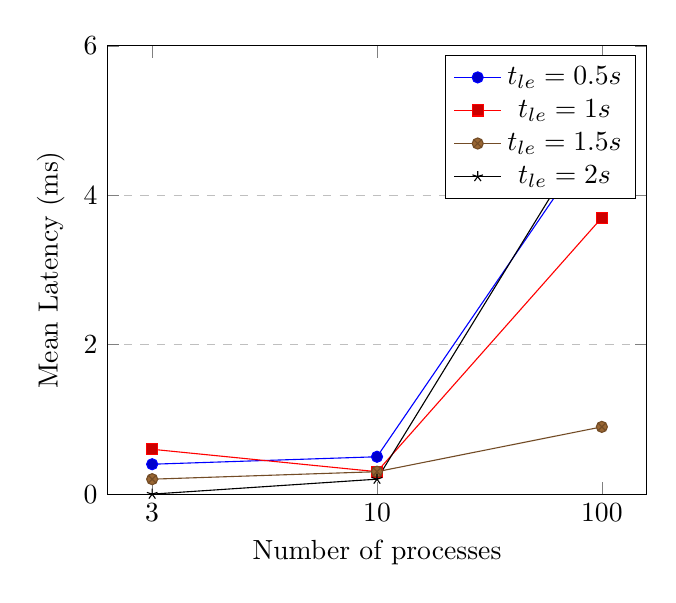
\begin{tikzpicture}
            \begin{axis}[
                    xlabel={Number of processes},
                    ylabel={Mean Latency (ms)},
                    xtick=data,
                    symbolic x coords={3, 10, 100},
                    ymin=0, ymax=6,
                    ymajorgrids=true,
                    grid style=dashed
                ]
                \addplot coordinates {(3, 0.4) (10, 0.5) (100, 4.9)};
                \addlegendentry{$t_{le} = 0.5s$}
                \addplot coordinates {(3, 0.6) (10, 0.3) (100, 3.7)};
                \addlegendentry{$t_{le} = 1s$}
                \addplot coordinates {(3, 0.2) (10, 0.3) (100, 0.9)};
                \addlegendentry{$t_{le} = 1.5s$}
                \addplot coordinates {(3, 0.0) (10, 0.2) (100, 5.1)};
                \addlegendentry{$t_{le} = 2s$}
            \end{axis}
        \end{tikzpicture}
        \caption{Mean latency comparison for $\alpha = 0$}
    \end{subfigure}%
    \begin{subfigure}{.55\textwidth}
        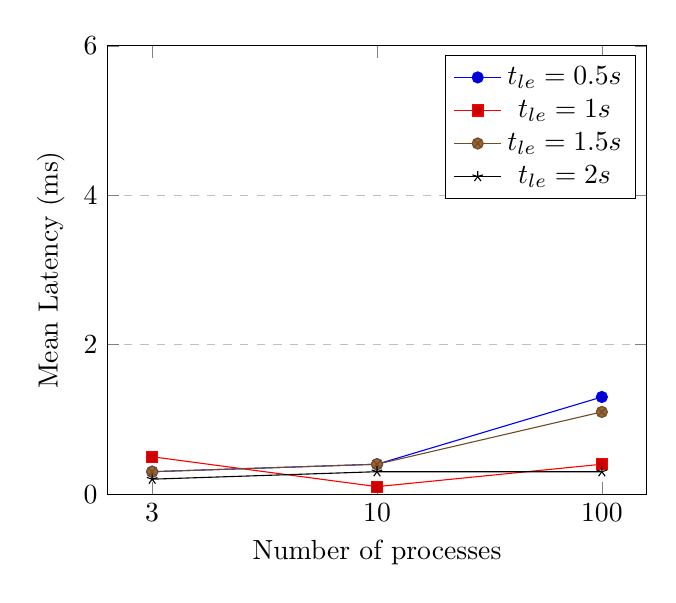
\begin{tikzpicture}
            \begin{axis}[
                    xlabel={Number of processes},
                    ylabel={Mean Latency (ms)},
                    xtick=data,
                    symbolic x coords={3, 10, 100},
                    ymin=0, ymax=6,
                    ymajorgrids=true,
                    grid style=dashed
                ]
                \addplot coordinates {(3, 0.3) (10, 0.4) (100, 1.3)};
                \addlegendentry{$t_{le} = 0.5s$}
                \addplot coordinates {(3, 0.5) (10, 0.1) (100, 0.4)};
                \addlegendentry{$t_{le} = 1s$}
                \addplot coordinates {(3, 0.3) (10, 0.4) (100, 1.1)};
                \addlegendentry{$t_{le} = 1.5s$}
                \addplot coordinates {(3, 0.2) (10, 0.3) (100, 0.3)};
                \addlegendentry{$t_{le} = 2s$}
            \end{axis}
        \end{tikzpicture}
        \caption{Mean latency comparison for $\alpha = 0.1$}
    \end{subfigure}
    \begin{subfigure}{.55\textwidth}
        \vspace{1cm}
        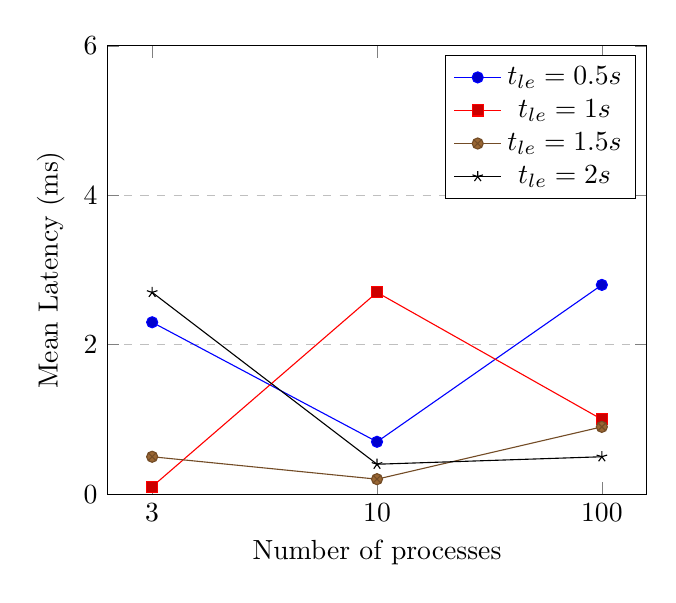
\begin{tikzpicture}
            \begin{axis}[
                    xlabel={Number of processes},
                    ylabel={Mean Latency (ms)},
                    xtick=data,
                    symbolic x coords={3, 10, 100},
                    ymin=0, ymax=6,
                    ymajorgrids=true,
                    grid style=dashed
                ]
                \addplot coordinates {(3, 2.3) (10, 0.7) (100, 2.8)};
                \addlegendentry{$t_{le} = 0.5s$}
                \addplot coordinates {(3, 0.1) (10, 2.7) (100, 1.0)};
                \addlegendentry{$t_{le} = 1s$}
                \addplot coordinates {(3, 0.5) (10, 0.2) (100, 0.9)};
                \addlegendentry{$t_{le} = 1.5s$}
                \addplot coordinates {(3, 2.7) (10, 0.4) (100, 0.5)};
                \addlegendentry{$t_{le} = 2s$}
            \end{axis}
        \end{tikzpicture}
        \caption{Mean latency comparison for $\alpha = 1$}
    \end{subfigure}
    \caption{Mean latency comparison for fixed timeout and alpha values and different number of processes}
\end{figure}
Since consensus is reached before the call to \textit{hold}, the differences in the \( t_{le} \) values do not significantly impact performance. In a larger system, having a timeout is very useful, because it allows the system to still be able to reach a consensus by reducing the number of proposing process to only one.
The choice of timeout should balance failure detection and system stability. A timeout that is too long delays the election of a new leader when a failure occurs, increasing recovery time. On the other hand, a well-chosen timeout ensures that the system remains responsive without unnecessary leader use.

\newpage

\subsection{Results for a fixed number of processes}
Let's first analyze the results for a fixed number of processes $N$ and different values of $t_{le}$.

\begin{figure}[h!]
    \centering
    \begin{subfigure}{0.55\textwidth}
        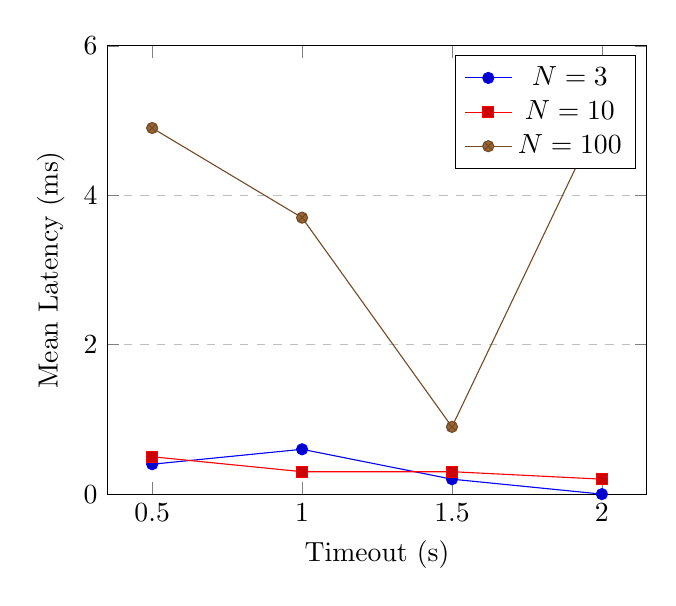
\begin{tikzpicture}
            \begin{axis}[
                    xlabel={Timeout (s)},
                    ylabel={Mean Latency (ms)},
                    xtick=data,
                    symbolic x coords={0.5, 1, 1.5, 2},
                    ymin=0, ymax=6,
                    ymajorgrids=true,
                    grid style=dashed
                ]
                \addplot coordinates {(0.5, 0.4) (1, 0.6) (1.5, 0.2) (2, 0.0)};
                \addlegendentry{$N = 3$}
                \addplot coordinates {(0.5, 0.5) (1, 0.3) (1.5, 0.3) (2, 0.2)};
                \addlegendentry{$N = 10$}
                \addplot coordinates {(0.5, 4.9) (1, 3.7) (1.5, 0.9) (2, 5.1)};
                \addlegendentry{$N = 100$}
            \end{axis}
        \end{tikzpicture}
        \caption{Mean latency comparison for $\alpha = 0$}
    \end{subfigure}%
    \begin{subfigure}{.55\textwidth}
        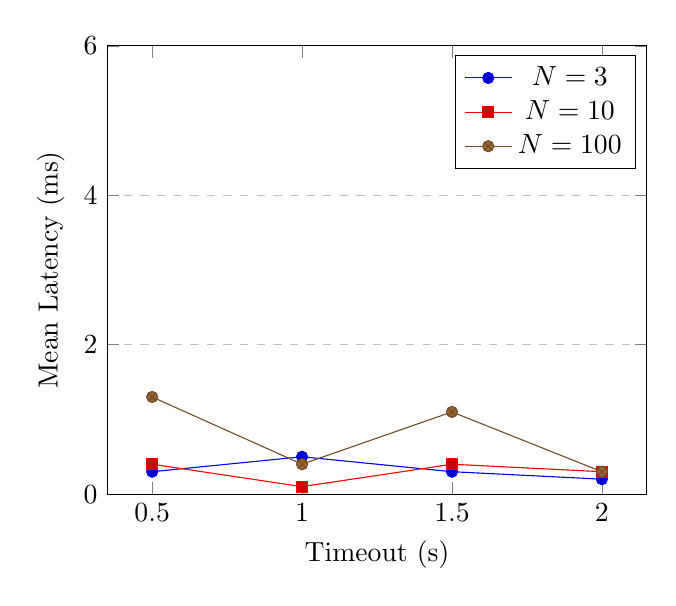
\begin{tikzpicture}
            \begin{axis}[
                    xlabel={Timeout (s)},
                    ylabel={Mean Latency (ms)},
                    xtick=data,
                    symbolic x coords={0.5, 1, 1.5, 2},
                    ymin=0, ymax=6,
                    ymajorgrids=true,
                    grid style=dashed
                ]
                \addplot coordinates {(0.5, 0.3) (1, 0.5) (1.5, 0.3) (2, 0.2)};
                \addlegendentry{$N = 3$}
                \addplot coordinates {(0.5, 0.4) (1, 0.1) (1.5, 0.4) (2, 0.3)};
                \addlegendentry{$N = 10$}
                \addplot coordinates {(0.5, 1.3) (1, 0.4) (1.5, 1.1) (2, 0.3)};
                \addlegendentry{$N = 100$}
            \end{axis}
        \end{tikzpicture}
        \caption{Mean latency comparison for $\alpha = 0.1$}
    \end{subfigure}
    \begin{subfigure}{.55\textwidth}
        \vspace{1cm}
        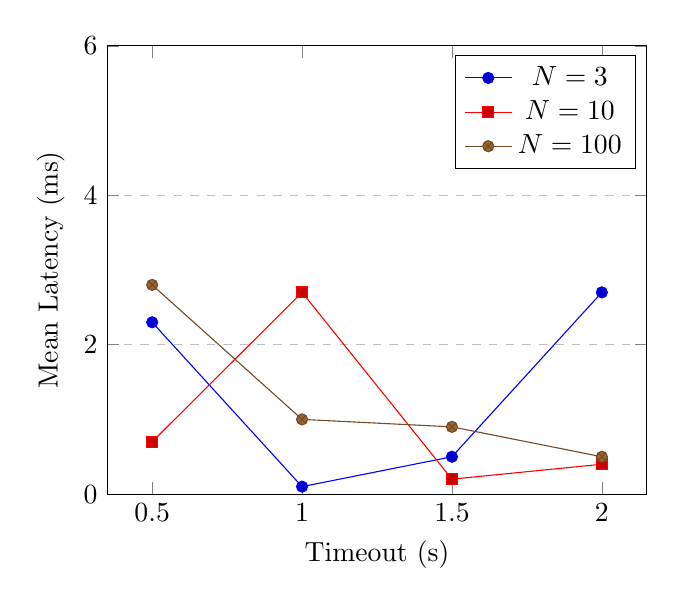
\begin{tikzpicture}
            \begin{axis}[
                    xlabel={Timeout (s)},
                    ylabel={Mean Latency (ms)},
                    xtick=data,
                    symbolic x coords={0.5, 1, 1.5, 2},
                    ymin=0, ymax=6,
                    ymajorgrids=true,
                    grid style=dashed
                ]
                \addplot coordinates {(0.5, 2.3) (1, 0.1) (1.5, 0.5) (2, 2.7)};
                \addlegendentry{$N = 3$}
                \addplot coordinates {(0.5, 0.7) (1, 2.7) (1.5, 0.2) (2, 0.4)};
                \addlegendentry{$N = 10$}
                \addplot coordinates {(0.5, 2.8) (1, 1.0) (1.5, 0.9) (2, 0.5)};
                \addlegendentry{$N = 100$}
            \end{axis}
        \end{tikzpicture}
        \caption{Mean latency comparison for $\alpha = 1$}
    \end{subfigure}
    \caption{Mean latency comparison for fixed number of processes and alpha values}
\end{figure}

We can see here that the latency increases as the number of processes grows. This is due to the required quorum size needed to reach consensus. However, while having fewer processes can be faster, it is hardly scalable for more general use cases where a high number of requests may occur. With too few processes, the system risks overloading. Furthermore, with more processes, and given that at least
$ \frac{N}{2} + 1$ correct processes are required, the system can tolerate a higher number of failures.

\newpage

\subsection{Results for the probability of failure}
Let's now analyze the results for fixed numbers of processes $N$ and timeout $t_{le}$, with different probabilities of failure $\alpha$.

\begin{figure}[h!]
    \begin{subfigure}{0.55\textwidth}
        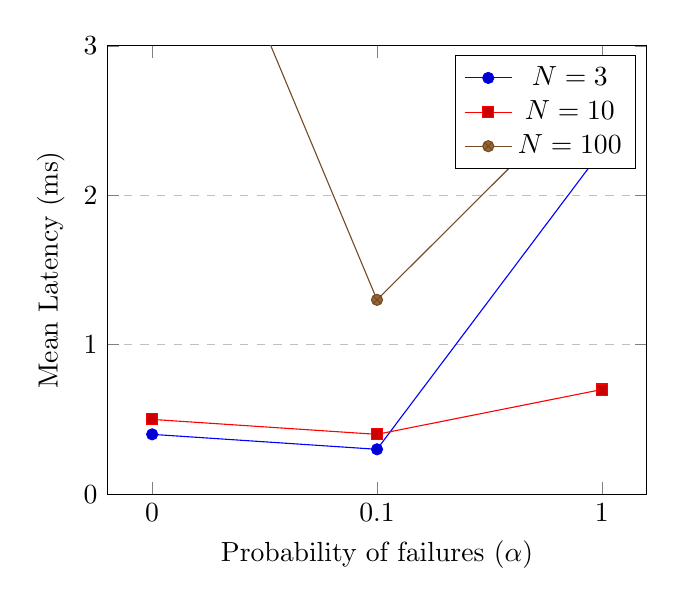
\begin{tikzpicture}
            \begin{axis}[
                    xlabel={Probability of failures ($\alpha$)},
                    ylabel={Mean Latency (ms)},
                    xtick=data,
                    symbolic x coords={0, 0.1, 1},
                    ymin=0, ymax=3,
                    ymajorgrids=true,
                    grid style=dashed
                ]
                \addplot coordinates {(0, 0.4) (0.1, 0.3) (1, 2.3)};
                \addlegendentry{$N = 3$}
                \addplot coordinates {(0, 0.5) (0.1, 0.4) (1, 0.7)};
                \addlegendentry{$N = 10$}
                \addplot coordinates {(0, 4.9) (0.1, 1.3) (1, 2.8)};
                \addlegendentry{$N=100$}
            \end{axis}
        \end{tikzpicture}
        \caption{Mean latency for $t_{le} = 0.5s$}

    \end{subfigure}%
    \begin{subfigure}{.55\textwidth}
        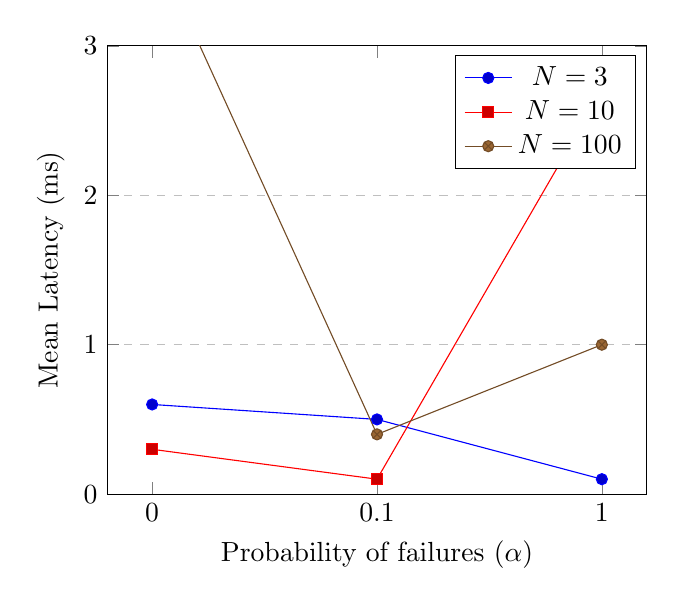
\begin{tikzpicture}
            \begin{axis}[
                    xlabel={Probability of failures ($\alpha$)},
                    ylabel={Mean Latency (ms)},
                    xtick=data,
                    symbolic x coords={0, 0.1, 1},
                    ymin=0, ymax=3,
                    ymajorgrids=true,
                    grid style=dashed
                ]
                \addplot coordinates {(0, 0.6) (0.1, 0.5) (1, 0.1)};
                \addlegendentry{$N = 3$}
                \addplot coordinates {(0, 0.3) (0.1, 0.1) (1, 2.7)};
                \addlegendentry{$N = 10$}
                \addplot coordinates {(0, 3.7) (0.1, 0.4) (1, 1.0)};
                \addlegendentry{$N=100$}
            \end{axis}
        \end{tikzpicture}

        \caption{Mean latency for $t_{le} = 1s$}
    \end{subfigure}
    \begin{subfigure}{.55\textwidth}
        \vspace{1cm}
        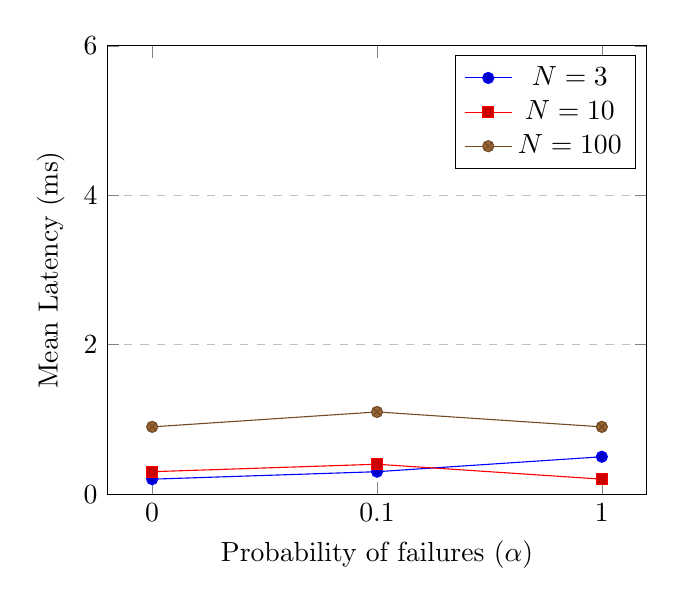
\begin{tikzpicture}
            \begin{axis}[
                    xlabel={Probability of failures ($\alpha$)},
                    ylabel={Mean Latency (ms)},
                    xtick=data,
                    symbolic x coords={0, 0.1, 1},
                    ymin=0, ymax=6,
                    ymajorgrids=true,
                    grid style=dashed
                ]

                \addplot coordinates {(0, 0.2) (0.1, 0.3) (1, 0.5)};
                \addlegendentry{$N = 3$}
                \addplot coordinates {(0, 0.3) (0.1, 0.4) (1, 0.2)};
                \addlegendentry{$N = 10$}
                \addplot coordinates {(0, 0.9) (0.1, 1.1) (1, 0.9)};
                \addlegendentry{$N = 100$}

            \end{axis}
        \end{tikzpicture}
        \caption{Mean latency for $t_{le} = 1.5s$}
    \end{subfigure}
    \begin{subfigure}{.55\textwidth}
        \vspace{1cm}
        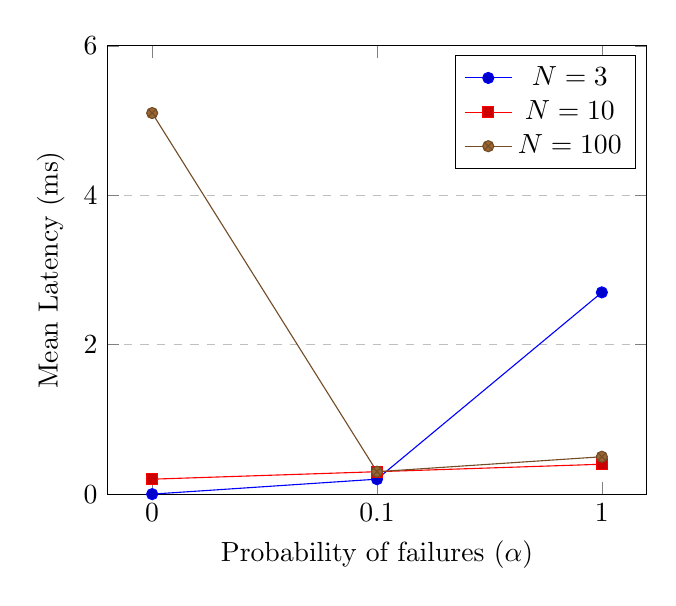
\begin{tikzpicture}
            \begin{axis}[
                    xlabel={Probability of failures ($\alpha$)},
                    ylabel={Mean Latency (ms)},
                    xtick=data,
                    symbolic x coords={0, 0.1, 1},
                    ymin=0, ymax=6,
                    ymajorgrids=true,
                    grid style=dashed
                ]

                \addplot coordinates {(0, 0.0) (0.1, 0.2) (1, 2.7)};
                \addlegendentry{$N = 3$}
                \addplot coordinates {(0, 0.2) (0.1, 0.3) (1, 0.4)};
                \addlegendentry{$N = 10$}
                \addplot coordinates {(0, 5.1) (0.1, 0.3) (1, 0.5)};
                \addlegendentry{$N = 100$}

            \end{axis}
        \end{tikzpicture}
        \caption{Mean latency for $t_{le} = 2s$}
    \end{subfigure}
    \caption{Mean latency comparison for fixed number of processes and alpha values}
\end{figure}

We can see in this part that the latency increases as the probability of failure
grows. This is due to the fact that the processes are more likely to fail, so they can't respond to reqyests and thus in order to reach a consensus, the process need to call all of the correct processes ($N/2 + 1$).
\end{document}
